
\chapter{Modeling and control of fixed-wing \acsp{uav} in uniform wind}\label{cha:fixed_wing_uav}
\section{Definitions and terminology}
Fixed-wind \acp{uav} are receiving increasing commercial and research interest, and offer a number of advantages in many usecases. In the following sections a thorough description of
general fixed-wing kinematics and control is presented, as well as a description of the specific platform used in this work. 
First, some common definitions and terminology are established. These definitions are 
 common in many other works related to fixed-wing aircraft, such as \cite{uav_dynamics_wind}. 

\subsection{Coordinate reference frames}
For \ac{uav} applications in wind, there are mainly four different coordinate frames that are relevant to consider: the inertial frame which is 
fixed in the earth, the air-relative frame, the body frame and the wind reference frame. The body frame and wind reference frames are related through the \textit{angle of attack} $\alpha$ and \textit{sideslip} $\beta$
 as shown in Figure \ref{fig:body_wind_frame}.
\begin{figure}
    \begin{center}
        \begin{tikzpicture}
            \coordinate (body) at ($(0,0)+(45:-.25)$);
            

            \draw[my_v] (body) -- node[at end, left]{$x$} (45:1.5);
            \draw[my_v] (body) -- node[at end, below]{$y$} (-45:1.5);

            \draw[my_v] (body) -- node[at end, left]{$x_{w}$} ++ (80:1.5);
            \draw[my_v] (body) -- node[at end, below]{$y_{w}$} ++ (-10:1.5);
            \draw[my_v] (body) -- node[at end, left]{$\airvec$} ++ (80:3);

            \draw[my_v] (.5,.5) arc(45:80:1) node[midway, anchor=225]{$\beta$};

            \Drone{0}{0}{50};
        \end{tikzpicture}
        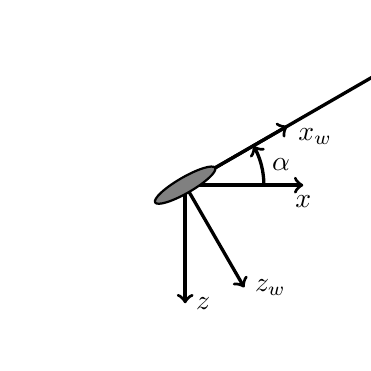
\begin{tikzpicture}
            \useasboundingbox (-2, -2) rectangle (2, 2);
            \coordinate (origin) at (0,0);

            \draw[my_v] (origin) -- node[at end, below]{$x$} ++ (1.5,0);
            \draw[my_v] (origin) -- node[at end, right]{$z$} ++ (0,-1.5);

            \draw[my_v] (origin) --node[at end, anchor=160]{$x_w$} ++ (30:1.5);
            \draw[my_v] (origin) --node[at end, right]{$z_w$} ++ (-60:1.5);
            \draw[my_v] (origin) --node[at end, anchor=160]{$\airvec$} ++ (30:3);

            \draw[rotate=30,thick,fill=gray] (origin) ellipse (0.44 and 0.1);

            \draw[my_v] (1,0) arc(0:30:1) node[midway, anchor=180]{$\alpha$};
        \end{tikzpicture}
    \end{center}
    \caption{Relation between body and wind frames}
    \label{fig:body_wind_frame}
\end{figure}

\begin{definition}[Inertial frame]
    The earth-fixed frame, which for the purposes in this thesis can be considered inertial, is denoted with subscript $I$.
    A position vector in the inertial frame is defined in the \ac{ned} order as
    \begin{equation}
        \vec{p}_I = (x_N, y_E, -h)
    \end{equation}
    where $x_N$ points in the north direction, $y_E$ points east and $h$ is the altitude above the ground,
    in order to form a right-handed coordinate system.
\end{definition}

\begin{definition}[Air frame]
    The air frame, denoted with subscript $A$, is fixed at any point in the air and aligned with the current direction of wind. In the case of non-zero wind,
    this coordinate frame moves with the same speed as the earth-relative wind at the frames origin.
    This means that inertial frame coordinates become time-dependent in the air frame, and are given by
    \begin{align}
        x_{N,A}(t) &= \cos\winddir x_{N,I} + \sin\winddir y_{E,I} - Wt\\
        y_{E,A}(t) &= -\sin\winddir x_{N,I} + \cos\winddir y_{E,I}
    \end{align}
    where $\windspd$ is the wind speed and $\winddir$ the wind direction.
\end{definition}

\begin{definition}[Body frame]
    The body frame, denoted with subscript $B$ is fixed in the \ac{uav} center of gravity.
    A position vector in the body frame is defined as
    \begin{equation}
        \vec{p}_B = (x, y, z)
    \end{equation}
    where $x$ axis points forward through the \ac{uav}, $y$ points to the right and $z$ points down.
\end{definition}

\begin{definition}[Wind reference frame]
    The wind reference frame, denoted with subscript $\windspd$ is related to the current direction of motion
    through the air.
    A position vector in the wind reference frame is defined as
    \begin{equation}
        \vec{p}_W = (x_w, y_w, z_w)
    \end{equation}
    where the $x_w$ axis points in the same direction as the velocity through the air $\airvec$, 
    $y_w$ points to the right of $x_w$ and $z$ points down relative $x_w$ and $y_w$.
\end{definition}

\subsection{Attitude representation}
The attitude of the \ac{uav} is represented by the \textit{Euler angles}. 

\begin{definition}[Euler angles]
The Euler angle vector is defined as
\begin{equation}
    \vec{\Phi}=(\phi, \theta, \psi)
\end{equation}
where the \textit{roll angle} $\phi$ is rotation around the north inertial axis, 
the \textit{pitch angle} $\theta$ is rotation around the east inertial axis and
the \textit{yaw angle} $\psi$ is rotation around the downwards inertial axis. The yaw angle is often 
referred to as \textit{heading} in this thesis.

The relationship between coordinates in the body frame and inertial frame is given
in \cite{sensor_fusion} as the rotation matrix 

\begin{equation}\label{eq:r_i_b}
\mathcal{R}^I_B = \mathcal{R}^x_\phi\mathcal{R}^y_\theta\mathcal{R}^z_\psi\\
=
\begin{bmatrix}
    1 & 0 & 0 \\
    0 & \cos\phi & \sin\phi \\
    0 & -\sin\phi & \cos\phi
\end{bmatrix}
\begin{bmatrix}
    \cos\theta & 0 & -\sin\theta \\
    0 & 1 & 0 \\
    \sin\theta & 0 & \cos\theta
\end{bmatrix}      
\begin{bmatrix}
    \cos\psi & \sin\psi & 0 \\
    -\sin\psi & \cos\psi & 0 \\
    0 & 0 & 1
\end{bmatrix}
\end{equation}  
\end{definition}

\noindent Note that this attitude representation is not uniquely defined for $\theta=\pm\pi/2$. However, this is not an issue since such angles 
never occur in the situations studied in this thesis.
\begin{figure}
    \centering
    \includegraphics[scale=0.25]{parrot}
    \caption{\ac{uav} platform used for real flight experiments}
    \label{fig:parrot}
\end{figure}
\subsection{Fixed-wing \ac{uav}}
A fixed-wing \ac{uav} is, in general, equipped with two horizontal wings that are fixed in the body frame.
In order to stay in the air, the forward velocity relative to the air must be above a certain threshold, \ie
\begin{equation}
    V > V_{s}
\end{equation}
where $V_s$ is the airframe-dependent \textit{stall speed}. In order to navigate through the
air, it is equipped with some or all of the following control surfaces:
\begin{itemize}
    \item \textit{Ailerons} to primarily control $\phi$.
    \item \textit{Elevators} to primarily control $\theta$.
    \item \textit{Rudders} to primarily control $\psi$.
\end{itemize}
The \ac{uav} is also equipped with one or several engines that are used to create the thrust which
increases the total energy of the system. In the case of a propeller-equipped aircraft, these might be facing towards or against the direction of motion.
The \ac{uav} platform used during real flight experiments in this work consists of a modified Parrot Disco airframe which is shown in Figure \ref{fig:parrot}.


\section{Wind field definition}
The wind field is commonly defined as a time and spatially dependent vector field \cite{wind_direct_computation}
\begin{equation}
    \windvec(x_N,y_E,h,t)=
    \begin{bmatrix}
        w_N(x_N,y_E,h,t) \\
        w_E(x_N,y_E,h,t) \\
        w_H(x_N,y_E,h,t)
    \end{bmatrix}
    .
\end{equation}
In this thesis, the vertical component $w_H$ will be neglected and the wind velocity is written as 
\begin{equation}
    \windvec=\windspd\begin{bmatrix}
        \cos\winddir\\
        \sin\winddir
    \end{bmatrix}
\end{equation}
where $\windspd$ is the wind magnitude and $\winddir$ is the wind direction. 
As mentioned in Section \ref{sec:aims} the wind is assumed constant and the dependencies on time and location are hence removed.
The wind field can be decomposed as
\begin{equation}
    \windvec = \bar{\windvec} + \windvec_s
\end{equation}
where $\bar{\windvec}$ is the mean wind field and $\windvec_s$ is described by some stochastic process. The random component is not considered in this thesis, \ie, it is assumed that $\windvec=\bar{\windvec}$.

\section{Wind estimation}
Wind field estimation techniques are important in order to handle the effects of winds on both planning and control of \acp{uav}.

\subsection{Direct computation of wind field}
When flying in non-zero wind, the resulting velocity relative to the earth is dependent on the velocity 
of the \ac{uav} relative to the air, $\airvec$, as well as the wind velocity $\windvec$.
This relationship, which is sometimes referred to as the \textit{wind triangle} is illustrated in Figure~\ref{fig:wind_triangle}. The 
velocity relative to the earth is given by 
\begin{equation}\label{eq:inertial_vel}
    \vel =\airvec + \windvec = \airspd\begin{bmatrix}
        \cos\psi \\
        \sin\psi
    \end{bmatrix}
    + \windspd\begin{bmatrix}
        \cos\winddir\\
        \sin\winddir
    \end{bmatrix}
    .
\end{equation}

\begin{figure}
    \begin{center}
        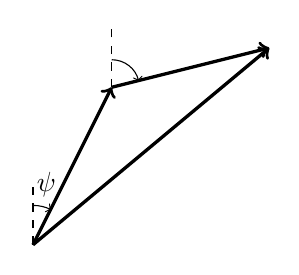
\begin{tikzpicture}
            \Drone{0}{0}{60};
            \draw[my_v](0,0) -- node[near end, left]{$\airvec$} (1, 2);
            \draw[my_v](1,2) -- node[near end, above]{$\windvec$} (3, 2.5); 
            \draw[my_v](0,0) -- node[midway, anchor=135]{$\vel$} (3, 2.5);

            \draw[dashed] (0,0) -- (0,0.75);
            \draw[->] (0,0.5) arc(90:62:0.5) node[midway, anchor=260]{$\psi$};

            \draw[dashed] (1,2) -- ++ (0,0.75);
            \draw[->] (1,2.35) arc(90:12:0.35) node[midway, anchor=235]{$\winddir$};
        \end{tikzpicture}
    \end{center}
    \caption{Relationship between velocities relative to the air and the earth}
    \label{fig:wind_triangle}    
\end{figure}
If it can be measured, \eg\ with the \ac{gps} of the \ac{uav}, the wind vector can be 
computed directly as 
\begin{equation}
    \windvec = \vel - \airvec
\end{equation}
where $\airvec$ can be measured as described in Section \ref{sec:measure_airspd}.
Assuming level flight, \ie\ $\theta\approx0$, it is shown in \cite{wind_direct_computation} that the measurement variance is
\begin{equation}
    e^2=\sigma_{\dot{x}_N}^2+\sigma_{\dot{y}_E}^2+\sigma_{\dot{z}_H}^2+\sigma_{\airspd}^2 + \airspd^2(\sigma_{\theta}^2+\sigma_{\alpha}^2+\sigma_{\beta}^2+\sigma_{\psi}^2)
\end{equation}
if this method is used. In standard unaided \ac{gps} systems, the standard deviation is approximately 0.1 m/s. Assuming the measurement variance of $\airspd$ is 0.2 m/s and angles 
can be measured up to $1\degree$ precision, the variance becomes $e^2=0.07+0.0012V_a^2$. If $\airspd=16$ m/s this corresponds to a standard deviation of 
$e=0.61$ m/s.
\subsection{Estimation using Extended Kalman Filter}\label{sec:wind_ekf}
A more robust approach is to use an \ac{ekf} to measure vehicle states. These are 
commonly used in autonomous systems to fuse measurements from many different sensors such as a \ac{gps}, \ac{imu} and barometer. 
A thorough reference on the underlying theory of \acp{ekf} is given in \cite{sensor_fusion}.

\subsection{Airspeed measurement}\label{sec:measure_airspd}
Fixed-wing \acp{uav} are often equipped with a \textit{pitot-tube} sensor to measure $\airspd=\|\airvec\|$.
Such a sensor consists of a metallic tube together with a sensor which measures the dynamic pressure $\Delta P$ of 
the air which flows through the tube. This measurement is related to the velocity of the air flow $V_{\text{pitot}}$ through 
Bernoulli's Equation as 
\begin{equation}
    V^2_{\text{pitot}} = K\frac{2\Delta P}{\rho}
\end{equation}
where $\rho$ is the density of the air. $K$ is a correction factor which compensates for calibration errors and 
generalizations such as assuming a perfect gas and constant temperature. Assuming that the sensor is mounted 
along the $x$ axis in the body frame, the relationship between $\airspd$ and $V_{\text{pitot}}$ is given in \cite{pitot} as
\begin{equation}
    \airspd^2=\frac{V^2_{\text{pitot}}}{\cos\alpha\cos\beta}=\frac{2K\Delta P}{\rho\cos\alpha\cos\beta}.
\end{equation}  

\section{Trajectory following}
To allow autonomous operation of an \ac{uav}, it needs to be equipped with a trajectory following controller.
The goal of this controller is to follow a pre-defined trajectory, which is defined by a set of 
line or curve segments in the inertial frame. This goal can be formulated as calculating the control signal 
in each time-step which minimizes the \textit{cross-track error}
\begin{equation}
    d(t)=\min\|\vec{p}_{I,\ac{uav}}(t)-\vec{p}_{I,\text{traj}}\|
\end{equation}
where $\vec{p}_{I,\text{traj}}$ is any point on the trajectory. 

\subsection{Kinematic model}
A kinematic model for fixed-wing \ac{uav} trajectory following in wind is introduced in \cite{uav_dynamics_wind} as, in the inertial frame:
\begin{align}\label{eq:traj_model}
    \dot{x}_N &= \airspd\cos\psi + \windspd\cos\winddir \\
    \dot{y}_E &= \airspd\sin\psi + \windspd\sin\winddir \\
    \dot{\psi} &= \frac{g}{\airspd}\tan\phi
\end{align}
where $\airspd$ is the speed relative to the air, $\psi$ is the heading and $\phi$ is the roll angle - both relative to the inertial frame.
Dynamics in the roll angle $\phi$ can be included as
\begin{align}
    \dot{\phi} = f_\phi(\phi-\phi_{\text{cmd}})
\end{align}
where $f_\phi$ is defined by the inner loop roll controller of the \ac{uav} and $\phi_{\text{cmd}}$ is the roll-angle command by the
trajectory following controller.

\subsection{Straight path following in wind}\label{sec:straight_path_wind}

\begin{figure}
    \begin{center}
        \tikzstyle{myaxis}=[
            ->,
            line width=1pt
            ]
            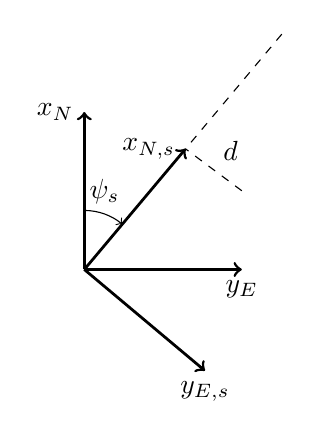
\begin{tikzpicture}
                \Drone{2}{1}{65}
                \coordinate (test) at (50:2);
                \draw[myaxis] (0, 0) -- node[at end, left]{$x_N$} (0, 2);
                \draw[myaxis] (0,0) -- node[at end, below]{$y_E$} (2, 0);

                \draw[myaxis] (0, 0) -- node[at end, left]{$x_{N,s}$} (test);
                \draw[myaxis] (0,0) -- node[at end, below]{$y_{E,s}$} (-40:2);
                \draw[->](0,0.75) arc(90:50:0.75) node[midway, above]{$\psi_s$};
                \draw[dashed](0, 0) -- (50:4);
                \draw[dashed](2,1) -- node[midway, anchor=south west]{$d$} (test);
            \end{tikzpicture}        
    \end{center}
    \caption{Coordinate frame for straight path following}
    \label{fig:coord_straight}
\end{figure}

To study the problem of accurately following a straight path segment in non-zero wind conditions, it is helpful to introduce another 
coordinate frame which is aligned with the path segment to follow, as shown in Figure \ref{fig:coord_straight}. The velocity vector relative to this frame, $\vec{v}_s$, is related to 
$\vel$ as
\begin{equation}
    \vec{v}_s=\begin{bmatrix}
        \cos\psi_s & \sin\psi_s \\
        -\sin\psi_s& \cos\psi_s
    \end{bmatrix}\vel
\end{equation}
which implies that
\begin{equation}
    \dot{d}\equiv\dot{y}_{E,s} = \airspd\sin(\psi-\psi_s) + \windspd\sin(\winddir-\psi_s).
\end{equation}
Assuming that $d=0$ and $\dot{d}=0$,
\begin{equation}
    \airspd\sin(\psi-\psi_s) + \windspd\sin(\winddir-\psi_s)=0.
\end{equation}
The cross-track error is thus minimized when
\begin{equation}\label{eq:wca}
    \psi=\wca\equiv-\arcsin\left(\frac{\windspd}{\airspd}\sin(\winddir-\psi_s)\right) + \psi_s.
\end{equation}
In the case of $\windspd=0$, this simplifies to $\wca=\psi_s$. In windy conditions, however, the wind 
has to be compensated with a constant offset which depends on wind speed, direction and the desired 
heading $\psi_s$. The angle $\wca$ is called the \textit{wind correction angle} \cite{uav_dynamics_wind}.

\subsection{Relationship between course and heading}
Since the direction of travel relative to the air and the ground generally differ, the concept of \textit{course} can instead be
introduced.

\begin{definition}[Course]
    The \ac{cog} is defined as 
    \begin{equation}\label{eq:cog}
        \cog = \atan2(V_E,V_N)
    \end{equation}
    where
    \begin{equation}
        V_N=\airspd\cos\psi + \windspd\cos\winddir
    \end{equation}
    and
    \begin{equation}
        V_E=\airspd\sin\psi + \windspd\sin\winddir
    \end{equation}
    \ie\ the north and east components of $\vel$.
\end{definition}


\section{ArduPlane autopilot}
The ArduPlane autopilot is an open source autopilot for fixed-wing \acp{uav} \cite{arduplane}. 
It contains high-level controllers for navigation, velocity and altitude control as well as 
low level logic to command the attitude and throttle of the vehicle. In the following section
the underlying theory of the components relevant for this thesis will be presented.

\subsection{Wind estimation}
The ArduPlane autopilot uses an \ac{ekf} to estimate $\windvec$. The implementation estimates 24 different states such as attitude, velocity, position, sensor biases and wind. The different process models and 
measurement equations are presented in \cite{px4_ecl_ekf}.

\subsection{Trajectory controller}\label{sec:traj_controller}
The ArduPlane autopilot uses the $L_1$ controller described in \cite{arduplane_l1} for trajectory following.
The goal of this controller is to follow a straight line from a start coordinate $\vec{p}_0$ to a goal
coordinate $\vec{p}_1$. This is obtained by aiming towards a point $P$ which is located at a
fixed distance $L_1$ from the \ac{uav}. 
The logic behind the controller is illustrated in Figure~\ref{fig:ss_defs},
where $\vec{p}$ is the \ac{uav} position and $\psi$ is the \ac{uav} heading.
\begin{figure}[htb]
    \begin{center}
    \tikzstyle{point} = [
        circle,
        minimum width=3.5pt,
        inner sep=0,
        fill=black
    ]
    \tikzstyle{my_v} = [
        ->,
        line width = 1.2pt
    ]
    \begin{tikzpicture}[scale=0.85]
        %\draw[help lines](0,0) grid (10,10);
        \coordinate (origin) at (1,1);
        \coordinate (drone) at (2,6);
        \coordinate (goal) at (9,9);
        \coordinate (ref) at (7,7);
        
        \node[anchor=300] at (drone) {$\vec{p}$};
        \draw[my_v] (drone) -- node[above, near end, anchor=south east]{$\vel$} ++ ({atan(2)}:2.5);

        \draw[->] (drone) -- node[right, at end]{$a_{\text{cmd}}$}++ (-45:1);

        \draw[->] ([yshift=0.7cm]drone) arc(90:{atan(2)}:0.7) node[above,midway]{$\psi$};
        \draw[dashed] (drone) --++ (0,1);
        \draw[->] (drone) ++ (0.5,1) arc({atan(2)}:{atan(0.2)}:{sqrt(1.25)}) node[midway,anchor=223]{$\eta$};
        

        \node[anchor=north west] at (origin) {$\vec{p}_0$};

        \node[anchor=north west] at (goal) {$\vec{p}_1$};
        
        \draw (drone) -- node[above,sloped]{$L_1$} (ref);
        \node[point] at (ref) {};
        \node[anchor=north west] at (ref) {$P$};
        
        \draw[] (origin) -- node[above, at end]{} (goal);
        \node[point] at (origin) {};
        \node[point] at (goal) {};
        \node[point] at (drone) {};
    
        \Drone{2}{6}{70};

    \end{tikzpicture}
        
    \caption{$L_1$ controller logic}
    \label{fig:ss_defs}
    \end{center}
\end{figure}

In the ArduPilot implementation, the distance $L_1$ is calculated as
\begin{equation}\label{eq:ardu_l1}
    L_1=\begin{cases}
        \frac{1}{\pi}\zeta\Delta TV & \mbox{if}\quad |\frac{1}{\pi}\zeta\Delta TV|>|\vec{p}_1-\vec{p}| \\
        |\vec{p}_1-\vec{p}| & \mbox{otherwise}
    \end{cases}
\end{equation}
where $V=|\vel|$, $\zeta$ is the damping factor and $\Delta T$ is the update period of the controller \cite{arduplane_l1}.
Using the speed relative to the inertial frame compensates for wind effects. In each time step, this controller corresponds to following a circular segment with radius
 \begin{equation}
    R=\frac{L_1}{2\sin\eta}
 \end{equation}
 which is tangent to $\vel$ in $\vec{p}$, where
 $\eta$ is defined as the angle between the \ac{uav} velocity vector $\vel$ and the line from the \ac{uav} to $P$. By introducing a line parallel to the line-segment from $\vec{p}_0$ to $\vec{p}_1$ the angle $\eta$ can be decomposed as
\begin{equation}\label{eq:eta_first}
    \eta=\eta_1+\eta_2
\end{equation}
where $\eta_2$ is defined as the angle from the velocity vector $\vel$ to this line.
The angle components are given by 
\begin{equation}
    \eta_2=\atan2(V_E\cos\psi_s - V_N\sin\psi_s,V_N\cos\psi_s+V_E\sin\psi_s)
\end{equation}
and 
\begin{equation}\label{eq:eta_last}
    \eta_1=\asin\left(\frac{x_N\sin\psi_s-y_E\cos\psi_s}{L_1}\right)
\end{equation}
where $\psi_s$ is the direction defined by the line from $\vec{p}_0$ to $\vec{p}_1$.
Finally, the circular segment is followed by issuing a lateral acceleration command
\begin{equation}\label{eq:lat_acc}
    a_{\text{cmd}}=2\frac{V^2}{L_1}\sin\eta
\end{equation}
The lateral acceleration command is translated to a roll command
\begin{equation}\label{eq:roll_cmd}
    \phi_{\text{cmd}}=\taninv(a_{\text{cmd}}/g)
\end{equation}
where $g$ is the gravitational constant. The low-level attitude controller is then used to track the desired roll.

In the case of a straight reference trajectory, it is shown in \cite{l1_controller} that \eqref{eq:lat_acc} 
is well approximated by its linearization
\begin{equation}
    a_{\text{cmd}}\approx2\frac{V}{L_1}\left(\dot{d}+\frac{V}{L_1}d\right)
\end{equation} 
which is a PD-controller. Furthermore, if inner-loop dynamics are neglected and 
$\vel$ is assumed to be parallel to the reference line, $a_{\text{cmd}}\approx \ddot{d}$ and
\begin{equation}
    \ddot{d} + 2\zeta\omega_n\dot{d} + \omega_n^2d=0
\end{equation}
with $\zeta=1/\sqrt{2}$ and $\omega_n=\sqrt{2}V/L_1$. This is a simple second-order system where 
the damping is constant, and the speed depends on the ratio between $V$ and $L_1$. 
\iffalse
\subsection{Altitude and velocity control loop}
ArduPlane uses a combined control loop to handle both desired altitude and velocity, called 
TECS (Total Energy Control System). This controller is based on the total energy of the \ac{uav},
which is defined as
\begin{equation}
    E_T=\frac{1}{2}mV^2 + mgh
\end{equation}
where $h$ is the altitude relative to the takeoff point. The total energy rate is derived
by taking the derivative with respect to time as
\begin{equation}
    \dot{E}_T=mV\dot{V} + mg\dot{h}
\end{equation}
The specific energy rate is then
\begin{equation}
    \dot{E}_S = \frac{\dot{E}_T}{mgV} = \frac{\dot{V}}{g} + \frac{\dot{h}}{V} = \frac{\dot{V}}{g} + \sin\gamma
\end{equation}
If $\gamma$ is small,
\begin{equation}
    \dot{E}_S\approx\frac{\dot{V}}{g} + \gamma
\end{equation} 
The longitudinal aircraft dynamics give
\begin{equation}
    T-D=\frac{\dot{V}}{g} + \gamma
\end{equation}
Thus, by increasing the thrust
energy is added to the system. By changing the pitch angle using the elevators, the balance 
between kinetic and potential energy can be modified. 
\fi

\subsection{Mission representation and flight modes}\label{sec:mission}
A \textit{mission} $\mathcal{M}$ is defined as 
\begin{equation}
    \mathcal{M} = \{\vec{p}_1, \hdots, \vec{p}_n\}
\end{equation}
\ie\  an ordered sequence of $n$ \textit{waypoints} represented as 
\begin{equation}
    \vec{p}=(x_N, y_E, h_{\text{rel}}, c_{\text{wp}})
\end{equation}
where $h_{\text{rel}}$ is the altitude relative to the takeoff position and $c_{\text{wp}}$ represents the mode of the waypoint. There are many different waypoint modes available
in ArduPlane, but this work will be focused on
\begin{equation}
    c_{\text{wp}}\in \{\text{Waypoint}, \text{Land}\}
\end{equation}
which are described below.
\subsubsection{Waypoint mode}
In \textit{waypoint} mode the trajectory following controller is used
to navigate along the line from $\vec{p}_0$ to $\vec{p}_1$. When $\vec{p}_1$ is reached, the flight mode
is updated depending on the next $c_{\text{wp}}$. A waypoint is assumed to have been reached when
\begin{equation}
    \|\vec{p}_{\text{rel}}-\vec{p}_{\text{wp}}\| < R_{\text{wp}}
\end{equation}
where $R_{\text{wp}}$ is defined by the user, or passed when
\begin{equation}
    \frac{\|\vec{p}_{\text{rel}}\cdot \vec{p}_{\text{wp}}\|}{\|\vec{p}_{\text{wp}}\|}
     \geq 1
\end{equation}
where $\vec{p}_{\text{rel}}=\vec{p}-\vec{p}_0$ and $\vec{p}_{\text{wp}}=\vec{p}_1-\vec{p}_0$ \cite{ardupilot_auto}.
\subsubsection{Land mode}
In \textit{Land} mode, the plane will attempt to land at a given coordinate. The landing procedure 
is divided into two different stages, the \textit{approach} stage and \textit{flare} stage.

During the approach stage, the \ac{uav} tries to accomplish the commanded \textit{glide slope}, which is
dependent on the previous waypoint position relative to the landing point. When the altitude decreases
below $\flarealt$, it enters the flare stage which means the throttle is completely turned off. 
During this stage the \ac{uav} will try to hold a target descent rate $\flaresink$ which is
defined by the user \cite{ardupilot_land}.